\section{6. Espectro electromagn\'etico de FM}

La norma técnica del Servicio de FM establece una marcada diferenciación entre las estaciones de alta y mediana potencia (categorías A, B, C y D) y las de baja potencia (E, F y G). Las primeras poseen radios de emisión máximos de 64, 50, 43 y 25 Km respectivamente, mientras que las segundas poseen rangos de servicio de tan solo 5, 3 y 1,5  Km cada una. La banda del espectro radioeléctrico comprendida entre las frecuencias de 88 MHz y 108 MHz es la correspondiente a las emisiones en FM. Está dividida en 100 canales siendo la frecuencia central del primer canal igual a $88,1 MHz$ y la del último $107,9MHz$. Para calcular la potencia a la que transmite una emisora de radio se utiliza la potencia radiada efectiva, la cual corresponde a Es la potencia suministrada a la antena multiplicada por su ganancia. Para determinarla deben considerarse las pérdidas en el sistema alimentador de antena. En la siguiente tabla aparece la clasifición de cada emisora según la PRE:



\begin{figure}[H]
    \centering
    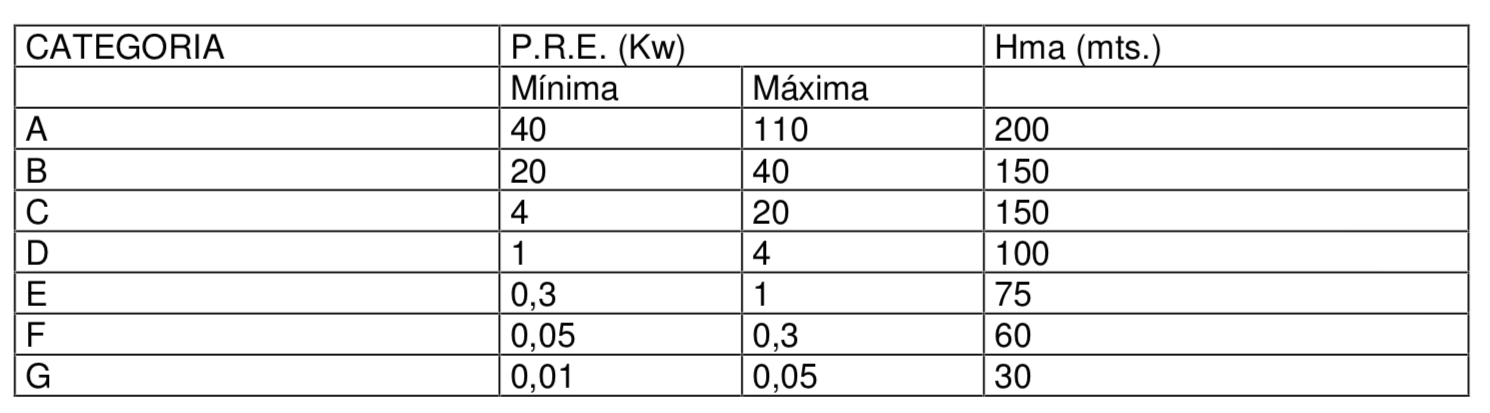
\includegraphics[scale=0.3]{Recursos/potencias.png}
    \caption{Tabla de potencias radidas efectivas Argentina}
\end{figure}

Se eligió la emisora de radio Los 40, cuya frecuencia central se encuentra en los $105,5MHz$ y se midió en el analizador de espectros la señal real:




\begin{figure}[H]
    \centering
    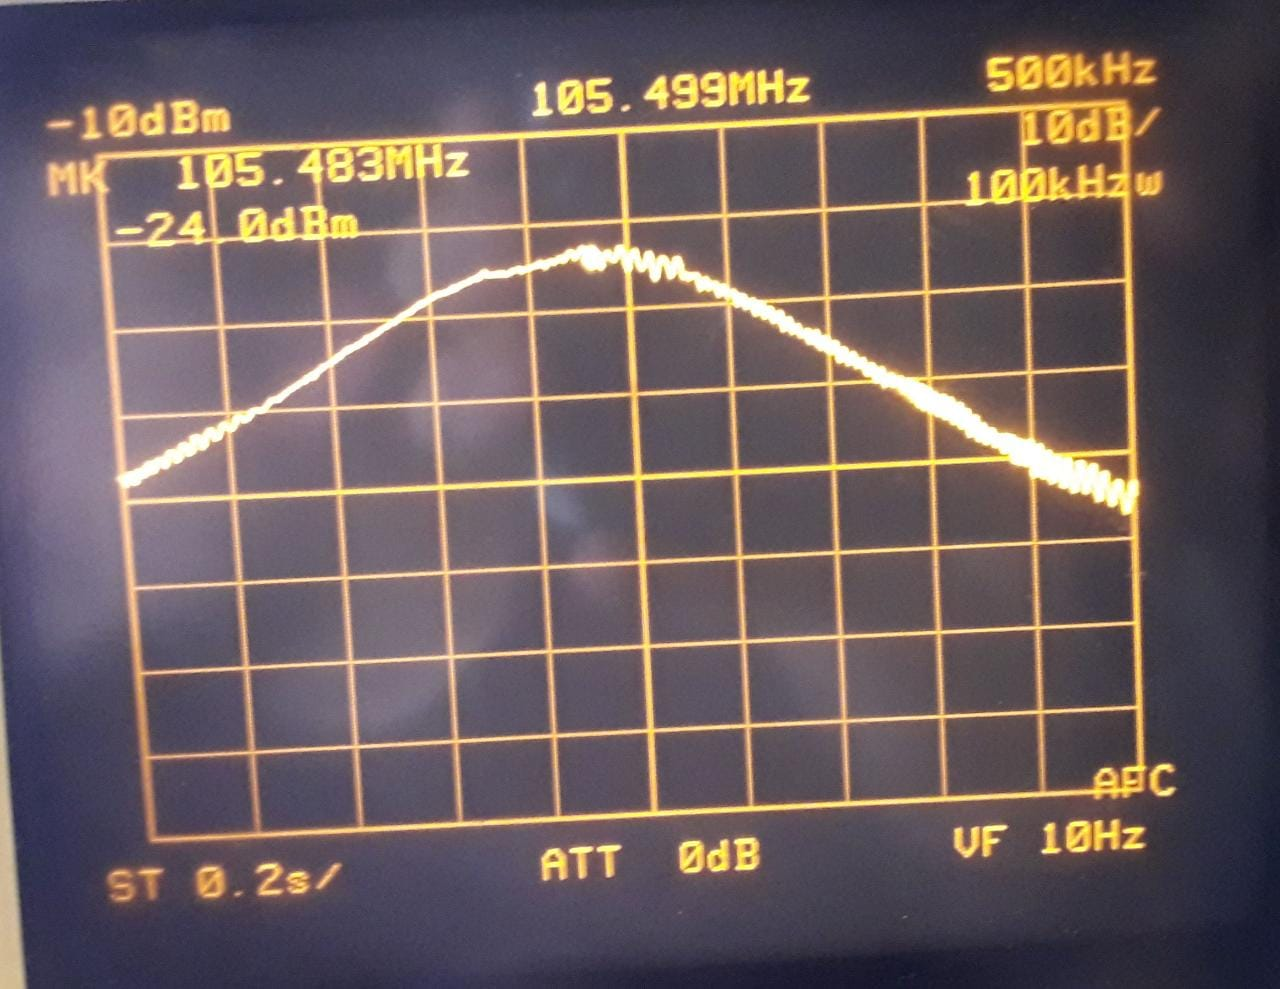
\includegraphics[scale=0.3]{Recursos/los40.jpeg}
    \caption{Tabla de potencias radidas efectivas Argentina}
\end{figure}

El centro de la banda de frecuencias se encuentra excatamente en los $105.5MHz$ como lo promociona la emisora. 